\section{Statistical Decision Theory}
%%%%%%%%%%%%%%%%%%%%%%%%%%%%%%%%%%%%%%%%%%%%%%%%%
\begin{frame}
  \frametitle{Decision Theoretic Preliminaries}

  \begin{block}{Parameter $\theta \in \Theta$}
    Unknown state of nature, from parameter space $\Theta$ 
  \end{block}

  \begin{block}{Observed Data}
    Observe $X$ with distribution $F_\theta$ from a sample space $\mathcal{X}$ 
  \end{block}

  \begin{block}{Estimator $\widehat{\theta}$}
    An estimator (aka a decision rule) is a function from $\mathcal{X}$ to $\Theta$
  \end{block}

  \begin{block}{Loss Function $L(\theta,\widehat{\theta})$}
    A function from $\Theta \times \Theta$ to $\mathbb{R}$ that gives the cost we incur if we report $\widehat{\theta}$ when the true state of nature is $\theta$.
  \end{block}

  
\end{frame}
%%%%%%%%%%%%%%%%%%%%%%%%%%%%%%%%%%%%%%%%%%%%%%%%%
\begin{frame}
  \frametitle{Examples of Loss Functions}

  \begin{table}
    \centering
    \begin{tabular}{ll}
      $L(\theta, \widehat{\theta}) = ( \theta - \widehat{\theta})^2$ & squared error loss\\
      $L(\theta, \widehat{\theta}) = |\theta - \widehat{\theta}|$ & absolute error loss\\
      %$L(\theta, \widehat{\theta}) = |\theta - \widehat{\theta}|^p$ & $L_p$ loss\\
      $L(\theta, \widehat{\theta}) = 0$ if $\theta = \widehat{\theta}$, 1 otherwise & zero-one loss \\ 
      $L(\theta, \widehat{\theta}) = \int \log \left[ \frac{f(x|\theta)}{f(x|\widehat{\theta})} \right] f(x|\theta)\, dx$ & Kullback--Leibler loss\\
    \end{tabular}
  \end{table}


\end{frame}
%%%%%%%%%%%%%%%%%%%%%%%%%%%%%%%%%%%%%%%%%%%%%%%%%
\begin{frame}
  \frametitle{(Frequentist) Risk of an Estimator $\widehat{\theta}$}

  \[
    \boxed{
      R(\theta, \widehat{\theta}) = \mathbb{E}_\theta \left[ L(\theta, \widehat{\theta}) \right] = \int L\big(\theta, \widehat{\theta}(x)\big) dF_\theta(x)}
  \]
  
  \vspace{1em}

  \begin{quote}
    The frequentist decision theorist seeks to evaulate, for each $\theta$, how much he would ``expect'' to lose if he used $\widehat{\theta}(X)$ repeatedly with varying $X$ in the problem.\\ \hfill (Berger, 1985)
  \end{quote}


  \begin{block}{Example: Squared Error Loss}
    $R(\theta, \widehat{\theta}) = \mathbb{E}_\theta\left[ (\theta - \widehat{\theta})^2 \right] = \mbox{MSE} = \mbox{Var}(\widehat{\theta}) + \mbox{Bias}_\theta^2(\widehat{\theta})$
  \end{block}

\end{frame}
%%%%%%%%%%%%%%%%%%%%%%%%%%%%%%%%%%%%%%%%%%%%%%%%%
\begin{frame}
  \frametitle{Bayes Risk and Maximum Risk}

  \begin{block}{Comparing Risk}
    $R(\theta, \widehat{\theta})$ is a \emph{function} of $\theta$ rather than a single number.
    We want an estimator with low risk, but how can we compare?
  \end{block}

  \vspace{1em}

  \begin{block}{Maximum Risk}
    \vspace{-1em}
    \[\boxed{\bar{R}(\widehat{\theta}) = \sup_{\theta \in \Theta} R(\theta, \widehat{\theta})}\] 
  \end{block}

  \vspace{-2em}

  \begin{block}{Bayes Risk}
    \vspace{-1em}
    \[\boxed{r(\pi, \widehat{\theta}) = \mathbb{E}_\pi \left[ R(\theta, \widehat{\theta}) \right], \mbox{ where } \pi \mbox{ is a prior for } \theta}\]
  \end{block}

\end{frame}
%%%%%%%%%%%%%%%%%%%%%%%%%%%%%%%%%%%%%%%%%%%%%%%%%
\begin{frame}
  \frametitle{Bayes and Minimax Rules}
  \framesubtitle{Minimize the Maximum or Bayes risk over all estimators $\widetilde{\theta}$}

  \begin{block}{Minimax Rule/Estimator}
    $\widehat{\theta}$ is \alert{minimax} if \hspace{0.5em} $\boxed{\displaystyle\sup_{\theta \in \Theta} R(\theta, \widehat{\theta}) = \displaystyle\inf_{\widetilde{\theta}} \sup_{\theta \in \Theta} R(\theta, \widetilde{\theta})}$

    \vspace{1em}

  \end{block}
  \begin{block}{Bayes Rule/Estimator}
    $\widehat{\theta}$ is a \alert{Bayes rule} with respect to prior $\pi$ if \hspace{0.5em} $\boxed{r(\pi, \widehat{\theta}) = \displaystyle\inf_{\widetilde{\theta}} r(\pi, \widetilde{\theta})}$
  \end{block}

\end{frame}
%%%%%%%%%%%%%%%%%%%%%%%%%%%%%%%%%%%%%%%%%%%%%%%%%
\begin{frame}
  \frametitle{Recall: Bayes' Theorem and Marginal Likelihood}
  Let $\pi$ be a prior for $\theta$.
  By Bayes' theorem, the \alert{posterior} $\pi(\theta|\mathbf{x})$ is
  \[
    \pi(\theta|\mathbf{x}) = \frac{f(\mathbf{x}|\theta)\pi(\theta)}{m(\mathbf{x})}
  \]
  where the \alert{marginal likelihood} $m(\mathbf{x})$ is given by
  \[
    m(\mathbf{x}) = \int f(\mathbf{x}|\theta) \pi(\theta)\, d\theta
  \]
\end{frame}
%%%%%%%%%%%%%%%%%%%%%%%%%%%%%%%%%%%%%%%%%%%%%%%%%
\begin{frame}
  \frametitle{Posterior Expected Loss}

  \begin{block}{Posterior Expected Loss}
    $\rho\big(\pi(\theta|\mathbf{x}), \widehat{\theta}\,\big) = \displaystyle \int L\big(\theta, \widehat{\theta}\,\big) \pi(\theta|\mathbf{x})\, d\theta$ 
  \end{block}

  \begin{block}{Bayesian Decision Theory} 
    Choose an estimator that minimizes posterior expected loss.
  \end{block}

  \begin{block}{Easier Calculation}
    Since $m(\mathbf{x})$ does not depend on $\theta$, to minimize $\rho\big(\pi(\theta|\mathbf{x}),\widehat{\theta}\,\big)$ it suffices to minimize $\int L(\theta, \widehat{\theta}) f(\mathbf{x}|\theta)\pi(\theta)\, d\theta$.
  \end{block}

  \begin{alertblock}{Question}
    Is there a relationship between Bayes risk, $r(\pi, \widehat{\theta}) \equiv\mathbb{E}_\pi[R(\theta, \widehat{\theta})]$, and posterior expected loss?
  \end{alertblock}

\end{frame}
%%%%%%%%%%%%%%%%%%%%%%%%%%%%%%%%%%%%%%%%%%%%%%%%%
\begin{frame}
  \frametitle{Bayes Risk vs.\ Posterior Expected Loss}
  \begin{block}{Theorem}
    $r(\pi, \widehat{\theta}) = \displaystyle\int \rho\big(\pi(\theta|\mathbf{x}), \widehat{\theta}(\mathbf{x})\big) m(\mathbf{x}) \, d\mathbf{x}$
  \end{block}

  \begin{block}{Proof}
    \vspace{-2em}
    \small
    \begin{eqnarray*}
      r(\pi,\widehat{\theta}) &=& \int R(\theta, \widehat{\theta}) \pi(\theta)\, d\theta = \int\left[ \int L\big(\theta, \widehat{\theta}(\mathbf{x})\big) f(\mathbf{x}|\theta)\, d\mathbf{x} \right]\pi(\theta)\, d\theta\\
      &=& \int \int L\big(\theta, \widehat{\theta}(\mathbf{x})\big) \left[f(\mathbf{x}|\theta)\pi(\theta)\right] \, d\mathbf{x}d\theta\\
      &=& \int \int L\big(\theta, \widehat{\theta}(\mathbf{x})\big) \left[\pi(\theta|\mathbf{x})m(\mathbf{x})\right] \, d\mathbf{x}d\theta\\
      &=& \int \left[\int L\big(\theta, \widehat{\theta}(\mathbf{x})\big) \pi(\theta|\mathbf{x}) \, d\theta \right] m(\mathbf{x})\, d\mathbf{x}\\
      &=& \int \rho\big(\pi(\theta|\mathbf{x}), \widehat{\theta}(\mathbf{x})\big) m(\mathbf{x}) \, d\mathbf{x}
    \end{eqnarray*}
  \end{block}
\end{frame}
%%%%%%%%%%%%%%%%%%%%%%%%%%%%%%%%%%%%%%%%%%%%%%%%%
\begin{frame}
  \frametitle{Finding a Bayes Estimator}

  \begin{block}{Hard Problem}
    Find the \alert{function} $\widehat{\theta}(\mathbf{x})$ that minimizes $r(\pi, \widehat{\theta})$.
  \end{block}

  \begin{block}{Easy Problem}
    Find the \alert{number} $\widehat{\theta}$ that minimizes $\rho\big(\pi(\theta|\mathbf{x}), \widehat{\theta})$
  \end{block}

  \begin{block}{Punchline}
    Since $r(\pi, \widehat{\theta}) = \displaystyle \int \rho\big(\pi(\theta|\mathbf{x}), \widehat{\theta}(\mathbf{x})\big) m(\mathbf{x}) \, d\mathbf{x}$, to minimize $r(\pi,\widehat{\theta})$ we can set $\widehat{\theta}(\mathbf{x})$ to be the value $\widehat{\theta}$ that minimizes $\rho\big(\pi(\theta|\mathbf{x}),\widehat{\theta})$.
  \end{block}

\end{frame}
%%%%%%%%%%%%%%%%%%%%%%%%%%%%%%%%%%%%%%%%%%%%%%%%%
\begin{frame}
  \frametitle{Bayes Estimators for Common Loss Functions}
  
  \begin{block}{Zero-one Loss}
    For zero-one loss, the Bayes estimator is the posterior mode.
  \end{block}

  \begin{block}{Absolute Error Loss: $L(\theta, \widehat{\theta}) = |\theta - \widehat{\theta}|$}
    For absolute error loss, the Bayes estimator is the posterior median.
  \end{block}

  \begin{block}{Squared Error Loss: $L(\theta, \widehat{\theta}) = (\theta - \widehat{\theta})^2$}
    For squared error loss, the Bayes estimator is the posterior mean.
  \end{block}
\end{frame}
%%%%%%%%%%%%%%%%%%%%%%%%%%%%%%%%%%%%%%%%%%%%%%%%%
\begin{frame}
  \frametitle{Derivation of Bayes Estimator for Squared Error Loss}

  By definition,
  \[
    \widehat{\theta} \equiv \underset{a \in \Theta}{\arg \min} \int (\theta - a)^2 \pi(\theta|\mathbf{x})\, d\theta
  \]
  Differentiating with respect to $a$, we have
  \begin{eqnarray*}
    2\int (\theta - a)\pi(\theta|\mathbf{x})\, d\theta &=& 0\\
    \int \theta \pi(\theta|\mathbf{x})\, d\theta &=& a
  \end{eqnarray*}

\end{frame}
%%%%%%%%%%%%%%%%%%%%%%%%%%%%%%%%%%%%%%%%%%%%%%%%%
\begin{frame}
  \frametitle{Example: Bayes Estimator for a Normal Mean}

  Suppose $X \sim N(\mu, 1)$ and $\pi$ is a $N(a, b^2)$ prior.
  Then,
  \footnotesize
  \begin{eqnarray*}
    \pi(\mu|x) &\propto& f(x|\mu) \times \pi(\mu)\\
    &\propto& \exp\left\{ -\frac{1}{2}\left[(x - \mu)^2  + \frac{1}{b^2}( \mu - a)^2\right]\right\} \\
   % &=& \exp\left\{ -\frac{1}{2}\left[\left(\mu^2 - 2\mu x + x^2\right)  + \frac{1}{b^2}\left( \mu^2 - 2\mu a + a^2\right)\right]\right\} \\
    &\propto& \exp\left\{ -\frac{1}{2}\left[\left( 1 + \frac{1}{b^2} \right)\mu^2 - 2 \left( x + \frac{a}{b^2} \right)\mu\right]\right\} \\
   % &=& \exp\left\{ -\frac{1}{2}\left[\left( \frac{b^2 + 1}{b^2} \right)\mu^2 - 2 \left( \frac{b^2 x + a}{b^2} \right)\mu\right]\right\} \\
   % &=& \exp\left\{ -\frac{1}{2}\left( \frac{b^2 + 1}{b^2} \right)\left[\mu^2 - 2 \left( \frac{b^2 x + a}{b^2 + 1} \right)\mu\right]\right\} \\
    &\propto& \exp\left\{ -\frac{1}{2}\left( \frac{b^2 + 1}{b^2} \right)\left[\mu - \left( \frac{b^2 x + a}{b^2 + 1} \right)\right]^2\right\}
  \end{eqnarray*}
  \normalsize

  So $\pi(\mu|x)$ is $N(m, \omega^2)$ with $\omega^2 = \frac{b^2}{1 + b^2}$ and $m = \omega^2 x + (1 - \omega^2) a$.
  Hence the Bayes estimator for $\mu$ under squared error loss is 
  \[
    \boxed{\widehat{\mathbf{\theta}}(X) = \frac{b^2X + a}{1 + b^2}}
  \]

\end{frame}
%%%%%%%%%%%%%%%%%%%%%%%%%%%%%%%%%%%%%%%%%%%%%%%%%
\begin{frame}
  \frametitle{Minimax Analysis}

  \small

  \begin{block}{Wasserman (2004)}
  \begin{quote}
    The advantage of using maximum risk, despite its problems, is that it does not require one to choose a prior.
  \end{quote}
  \end{block}

  \begin{block}{Berger (1986)}
  \begin{quote}
    Perhaps the greatest use of the minimax principle is in situations for which no prior information is available \dots but two notes of caution should be sounded. 
    First, the minimax principle can lead to bad decision rules\dots Second, the minimax approach can be devilishly hard to implement.
  \end{quote}
  \end{block}
\end{frame}
%%%%%%%%%%%%%%%%%%%%%%%%%%%%%%%%%%%%%%%%%%%%%%%%%
\begin{frame}
  \frametitle{Methods for Finding a Minimax Estimator}

  \begin{enumerate}
    \item Direct Calculation 
    \item Guess a ``Least Favorable'' Prior
    \item Search for an ``Equalizer Rule''
  \end{enumerate}

  \vspace{2em}
  \hfill\alert{Method 1 rarely applicable so focus on 2 and 3\dots}

\end{frame}
%%%%%%%%%%%%%%%%%%%%%%%%%%%%%%%%%%%%%%%%%%%%%%%%%
\begin{frame}
  \frametitle{The Bayes Rule for a Least Favorable Prior is Minimax}


  \begin{block}{Theorem}
    \small
    Let $\widehat{\theta}$ be a Bayes rule with respect to $\pi$ and suppose that for all $\theta\in \Theta$ we have $R(\theta,\widehat{\theta}) \leq r(\pi, \widehat{\theta})$.
    %\[
    %  \boxed{R(\theta,\widehat{\theta}) \leq r(\pi, \widehat{\theta})}
    %\]
    Then $\widehat{\theta}$ is a \textbf{minimax estimator}, and $\pi$ is called a \textbf{least favorable prior}.
  \end{block}

  \begin{block}{Proof}
    \small
    Suppose that $\widehat{\theta}$ is not minimax.
    Then there exists another estimator $\widetilde{\theta}$ with $\sup_{\theta\in\Theta} R(\theta, \widetilde{\theta}) < \sup_{\theta\in \Theta} R(\theta, \widehat{\theta})$.
    But since
    \[
      r(\pi, \widetilde{\theta}) \equiv \mathbb{E}_{\pi}\left[ R(\theta,\widetilde{\theta}) \right] \leq \mathbb{E}_{\pi}\left[ \sup_{\theta \in \Theta} R(\theta, \widetilde{\theta}) \right] = \sup_{\theta \in \Theta} R(\theta, \widetilde{\theta})
    \]
    but this implies that $\widehat{\theta}$ is \emph{not} Bayes with respect to $\pi$ since 
    \[
      r(\pi, \widetilde{\theta}) \leq \sup_{\theta\in \Theta} R(\theta, \widetilde{\theta}) < \sup_{\theta \in \Theta} R(\theta, \widehat{\theta}) \leq r(\pi, \widehat{\theta})
    \]
  \end{block}
\end{frame}
%%%%%%%%%%%%%%%%%%%%%%%%%%%%%%%%%%%%%%%%%%%%%%%%%
\begin{frame}
  \frametitle{Example of Least Favorable Prior}

  \begin{block}{Bounded Normal Mean}
  \begin{itemize}
    \item $X \sim N(\theta,1)$
    \item Squared error loss
    \item $\Theta = [-m,m]$ for $0 < m < 1$
  \end{itemize}
\end{block}

\begin{block}{Least Favorable Prior}
  $\pi(\theta) = 1/2$ for $\theta \in\{-m,m\}$, zero otherwise. 
\end{block}

\begin{block}{Resulting Bayes Rule is Minimax}
  \vspace{-1em}
\[
  \widehat{\theta}(X) = m \tanh(mX) = m\left[ \frac{\exp\left\{ mX \right\} - \exp\left\{ -mX \right\}}{\exp\left\{ mX \right\} + \exp\left\{ -mX \right\}}\right]
\]
\end{block}

\end{frame}
%%%%%%%%%%%%%%%%%%%%%%%%%%%%%%%%%%%%%%%%%%%%%%%%%
\begin{frame}
  \frametitle{Equalizer Rules}
  \begin{block}{Definition}
    An estimator $\widehat{\theta}$ is called an \textbf{equalizer rule} if its risk function is constant: $R(\theta, \widehat{\theta}) = C$ for some $C$.
  \end{block}

  \begin{block}{Theorem}
    If $\widehat{\theta}$ is an equalizer rule and is Bayes with respect to $\pi$, then $\widehat{\theta}$ is \textbf{minimax} and $\pi$ is \textbf{least favorable}.
  \end{block}
  
  \begin{block}{Proof}
    \vspace{-2em}
    \[
      r(\pi, \widehat{\theta}) = \int R(\theta, \widehat{\theta})\pi(\theta)\, d\theta = \int C \pi(\theta) \, d\theta = C 
    \]
    Hence, $R(\theta, \widehat{\theta}) \leq r(\pi, \widehat{\theta})$ for all $\theta$ so we can apply the preceding theorem. 
  \end{block}

\end{frame}
%%%%%%%%%%%%%%%%%%%%%%%%%%%%%%%%%%%%%%%%%%%%%%%%%
\begin{frame}
  \frametitle{Example: $X_1, \dots, X_n \sim \mbox{ iid Bernoulli}(p)$}

  Under a Beta$(\alpha, \beta)$ prior with  $\alpha = \beta = \sqrt{n}/2$, 
  \[
    \widehat{p} = \frac{n\bar{X} + \sqrt{n}/2}{n + \sqrt{n}}
  \]
  is the Bayesian posterior mean, hence the Bayes rule under squared error loss.
  The risk function of $\widehat{p}$ is,
  \[
    R(p, \widehat{p}) = \frac{n}{4(n + \sqrt{n})^2}
  \]
  which is constant in $p$.
  Hence, $\widehat{p}$ is an equalizer rule, and by the preceding theorem is minimax.


\end{frame}
%%%%%%%%%%%%%%%%%%%%%%%%%%%%%%%%%%%%%%%%%%%%%%%%%
\begin{frame}
  \frametitle{Problems with the Minimax Principle}
  \begin{columns}
    \column{0.48\textwidth}
    \begin{figure}
      \centering
      \footnotesize
      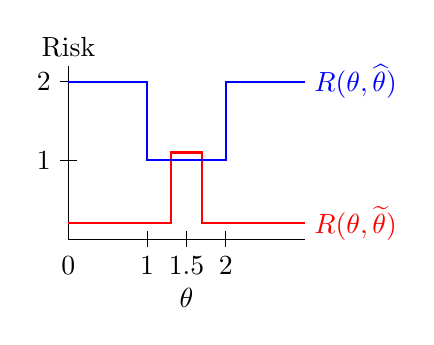
\begin{tikzpicture}
        \draw [-] (0,2.2) -- (0,0) -- (3,0);
        \node [above] at (0,2.2) {Risk};
        \node [below] at (1.5,-0.5) {$\theta$};
        \node [below] at (0,-0.1) {$0$};
        \foreach \x in {1,1.5,2}{
          \draw[xshift=\x cm] (0pt,-3pt) -- (0pt,3pt);
          \node[below] at (\x,-0.1) {\x}; 
        }
        \foreach \y in {1,2}{
          \draw[yshift=\y cm] (-3pt,0pt) -- (3pt,0pt);
          \node[left] at (-0.1,\y) {\y}; 
        }
        \draw [thick, color = red] (0,0.2) -- (1.3,0.2) -- (1.3,1.1) -- (1.7,1.1) -- (1.7,0.2) -- (3,0.2);
        \node [right, color = red] at (3,0.2) {$R(\theta, \widetilde{\theta})$};
        \draw [thick, color = blue] (0,2) -- (1,2) -- (1, 1) -- (2, 1) -- (2,2) -- (3,2);
        \node [right, color = blue] at (3,2) {$R(\theta, \widehat{\theta})$};
      \end{tikzpicture}
    \end{figure}

    \column{0.48\textwidth}
    \begin{figure}
      \footnotesize
      \centering
      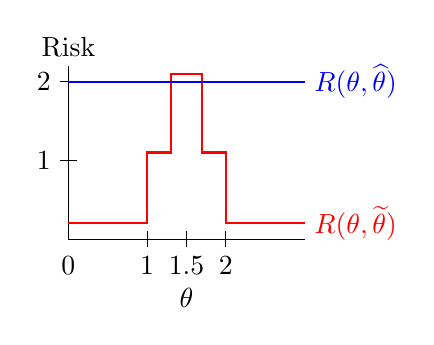
\begin{tikzpicture}
        \draw [-] (0,2.2) -- (0,0) -- (3,0);
        \node [above] at (0,2.2) {Risk};
        \node [below] at (1.5,-0.5) {$\theta$};
        \node [below] at (0,-0.1) {$0$};
        \foreach \x in {1,1.5,2}{
          \draw[xshift=\x cm] (0pt,-3pt) -- (0pt,3pt);
          \node[below] at (\x,-0.1) {\x}; 
        }
        \foreach \y in {1,2}{
          \draw[yshift=\y cm] (-3pt,0pt) -- (3pt,0pt);
          \node[left] at (-0.1,\y) {\y}; 
        }
        \draw [thick, color = red] (0,0.2) --(1,0.2) -- (1,1.1) -- (1.3,1.1) -- (1.3,2.1) -- (1.7,2.1) -- (1.7,1.1) -- (2,1.1) -- (2,0.2) -- (3,0.2);
        \node [right, color = red] at (3,0.2) {$R(\theta, \widetilde{\theta})$};
        \draw [thick, color = blue] (0,2) -- (3,2);
        \node [right, color = blue] at (3,2) {$R(\theta, \widehat{\theta})$};
      \end{tikzpicture}
    \end{figure}

  \end{columns}

  \vspace{2em}

  \small

  In the left panel, $\widetilde{\theta}$ is preferred by the minimax principle; in the right panel $\widehat{\theta}$ is preferred.
  But the only difference between them is that the right panel adds an additional \emph{fixed} loss of 1 for $1 \leq \theta \leq 2$.

  
\end{frame}
%%%%%%%%%%%%%%%%%%%%%%%%%%%%%%%%%%%%%%%%%%%%%%%%%
\begin{frame}
  \frametitle{Problems with the Minimax Principle}
  \small

  Suppose that $\Theta = \left\{ \theta_1, \theta_2 \right\}$, $\mathcal{A} = \left\{ a_1, a_2 \right\}$ and the loss function is:
  \begin{table}
    \centering
    \begin{tabular}{lrr}
      & $a_1$ & $a_2$ \\
      \cline{2-3}
      $\theta_1$ & \multicolumn{1}{|r|}{10} & \multicolumn{1}{r|}{10.01} \\
      \cline{2-3}
      $\theta_2$ & \multicolumn{1}{|r|}{8} & \multicolumn{1}{r|}{-8}\\
      \cline{2-3}
    \end{tabular}
  \end{table}
  
  \vspace{1em}

  \begin{itemize}
    \item Minimax principle: choose $a_1$
    \item Bayes: Choose $a_2$ unless $\pi(\theta_1) > 0.9994$
  \end{itemize}


  \vspace{1em}

  \alert{Minimax ignores the fact that under $\theta_1$ we can never do better than a loss of 10, and tries to prevent us from incurring a tiny additional loss of 0.01}

\end{frame}
%%%%%%%%%%%%%%%%%%%%%%%%%%%%%%%%%%%%%%%%%%%%%%%%%
%\begin{frame}
%
%  Regret and minimax regret.
%  And maybe Gamma-minimax, and gamma-minimax regret.
%\end{frame}
%%%%%%%%%%%%%%%%%%%%%%%%%%%%%%%%%%%%%%%%%%%%%%%%%%
\begin{frame}
  \frametitle{Dominance and Admissibility}

  \begin{block}{Dominance}
$\widehat{\theta}$ \textbf{dominates} $\widetilde{\theta}$ with respect to $R$ if $R(\theta,\widehat{\theta}) \leq R(\theta,\widetilde{\theta})$ for all $\theta \in \Theta$ and the inequality is strict for at least one value of  $\theta$. 
  \end{block}

  \begin{block}{Admissibility}
$\widehat{\theta}$ is \textbf{admissible} if no other estimator dominates it.
  \end{block}

  \begin{alertblock}{Inadmissiblility}
    $\widehat{\theta}$ is \textbf{inadmissible} if there is an estimator that dominates it. 
  \end{alertblock}

\end{frame}
%%%%%%%%%%%%%%%%%%%%%%%%%%%%%%%%%%%%%%%%%%%%%%%%%
\begin{frame}
  \frametitle{Example of an Admissible Estimator}


    Say we want to estimate $\theta$ from $X\sim N(\theta, 1)$ under squared error loss. 
    Is the estimator $\widehat{\theta}(X) = 3$ admissible?

    \vspace{2em}
    If not, then there is a $\widetilde{\theta}$ with $R(\theta,\widetilde{\theta}) \leq R(\theta,\widehat{\theta})$ for all $\theta$. 
    Hence:
    \[
      R(3, \widetilde{\theta}) \leq R(3, \widehat{\theta}) = \left\{\mathbb{E}\left[\widehat{\theta} - 3  \right] \right\}^2 + \mbox{Var}(\widehat{\theta}) = 0
    \]
    Since $R$ cannot be negative for squared error loss, 
    \[
      0 = R(3,\widetilde{\theta}) = \left\{ \mathbb{E}\left[ \widetilde{\theta} - 3 \right] \right\}^2 + \mbox{Var}(\widetilde{\theta})
    \]
    Therefore $\widehat{\theta} = \widetilde{\theta}$, so $\widehat{\theta}$ is admissible, although very silly!


\end{frame}
%%%%%%%%%%%%%%%%%%%%%%%%%%%%%%%%%%%%%%%%%%%%%%%%%
\begin{frame}
  \frametitle{Bayes Rules are Admissible}

  \begin{block}{Theorem A-1}
    Suppose that $\Theta$ is a discrete set and $\pi$ gives strictly positive probability to each element of $\Theta$.
    Then, if $\widehat{\theta}$ is a Bayes rule with respect to $\pi$, it is admissible.
  \end{block}

  \begin{block}{Theorem A-2}
    If a Bayes rule is unique, it is admissible.
  \end{block}

  \begin{block}{Theorem A-3}
    Suppose that $R(\theta, \widehat{\theta})$ is continuous in $\theta$ for all $\widehat{\theta}$ and that $\pi$ gives strictly positive probability to any open subset of $\Theta$. 
    Then if $\widehat{\theta}$ is a Bayes rule with respect to $\pi$, it is admissible.
  \end{block}

\end{frame}
%%%%%%%%%%%%%%%%%%%%%%%%%%%%%%%%%%%%%%%%%%%%%%%%%
\begin{frame}
  \frametitle{Admissible Equalizer Rules are Minimax}

  \begin{block}{Theorem}
    Let $\widehat{\theta}$ be an equalizer rule. 
    Then if $\widehat{\theta}$ is admissible, it is minimax.
  \end{block}
  \begin{block}{Proof}
    Since $\widehat{\theta}$ is an equalizer rule, $R(\theta, \widehat{\theta}) = C$.
    Suppose that $\widehat{\theta}$ is not minimax.
    Then there is a $\widetilde{\theta}$ such that

    \[
      \sup_{\theta \in \Theta} R(\theta,\widetilde{\theta}) < \sup_{\theta \in \Theta} R(\theta, \widehat{\theta}) = C
    \]

    But for any $\theta$, $R(\theta, \widetilde{\theta}) \leq \sup_{\theta \in \Theta} R(\theta, \widetilde{\theta})$.
    Thus we have shown that $\widetilde{\theta}$ dominates $\widehat{\theta}$, so that $\widehat{\theta}$ cannot be admissible.
  \end{block}
\end{frame}

%%%%%%%%%%%%%%%%%%%%%%%%%%%%%%%%%%%%%%%%%%%%%%%%%

\begin{frame}
  \frametitle{Minimax Implies ``Nearly'' Admissible}



  \begin{block}{Strong Inadmissibility}
    We say that $\widehat{\theta}$ is \textbf{strongly inadmissible} if there exists an estimator $\widetilde{\theta}$ and an $\varepsilon > 0$ such that $R(\theta, \widetilde{\theta}) < R(\theta, \widehat{\theta}) - \varepsilon$ for all $\theta$.
  \end{block}

  \begin{block}{Theorem}
    If $\widehat{\theta}$ is minimax, then it is \textbf{not} strongly inadmissible.
  \end{block}

\end{frame}

%%%%%%%%%%%%%%%%%%%%%%%%%%%%%%%%%%%%%%%%%%%%%%%%%
\begin{frame}
  \frametitle{Example: Sample Mean, Unbounded Parameter Space}

  \begin{block}{Theorem}
    Suppose that $X_1, \dots, X_n \sim N(\theta, 1)$ with $\Theta = \mathbb{R}$.
    Under squared error loss, one can show that $\widehat{\theta} = \bar{X}$ is admissible.
  \end{block}

  \begin{block}{Intuition}
    The proof is complicated, but effectively we view this estimator as a \textbf{limit} of a of Bayes estimator with prior $N(a, b^2)$, as $b^2 \rightarrow \infty$.
  \end{block}

  \begin{block}{Minimaxity}
    Since $R(\theta, \bar{X}) = \mbox{Var}(\bar{X}) = 1/n$, we see that $\bar{X}$ is an equalizer rule.
    Since it is admissible, it is therefore minimax.
  \end{block}

\end{frame}
%%%%%%%%%%%%%%%%%%%%%%%%%%%%%%%%%%%%%%%%%%%%%%%%%

\section{The James-Stein Estimator}
%%%%%%%%%%%%%%%%%%%%%%%%%%%%%%%%%%%%%%%%%%%%%%%%%
\begin{frame}
  \frametitle{Recall: Gauss-Markov Theorem}
  \begin{block}{Linear Regression Model}
    
    $$\mathbf{y} = X\beta + \boldsymbol{\epsilon}, \quad \mathbb{E}[\boldsymbol{\epsilon}|X] = \mathbf{0}$$
  \end{block}


  \begin{block}{Best Linear Unbiased Estimator}
    
    \begin{itemize}
      \item $\mbox{Var}(\epsilon|X) = \sigma^2 I \Rightarrow$ then OLS has lowest variance among linear, unbiased estimators of $\beta$.
      \item  $\mbox{Var}(\varepsilon|X)\neq \sigma^2 I \Rightarrow$ then GLS gives a lower variance estimator.  
    \end{itemize}
  \end{block}

  \begin{alertblock}{What if we consider biased estimators and squared error loss?}
    
  \end{alertblock}
    
\end{frame}
%%%%%%%%%%%%%%%%%%%%%%%%%%%%%%%%%%%%%%%%%%%%%%%%%
\begin{frame}
  \frametitle{Multiple Normal Means: $X \sim N(\theta, I)$}

  \begin{block}{Goal}
    Estimate the $p$-vector $\theta$ using $X$ with $L(\theta, \widehat{\theta}) = \lvert\lvert \widehat{\theta} - \theta\rvert\rvert^2$.
  \end{block}

  \begin{block}{Maximum Likelihood Estimator $\widehat{\theta}$}
MLE = sample mean, but only one observation: $\hat{\theta} = X$.
  \end{block}

  \begin{block}{Risk of $\widehat{\theta}$}
    
    \vspace{-1em}
\begin{equation*}
  \left( \hat{\theta} - \theta \right)' \left( \hat{\theta}- \theta \right) = \left( X - \theta \right)'\left( X-\theta \right)= \sum_{i = 1}^{p} \left( X_{i} - \theta_i \right)^2 \sim \chi^2_p 
\end{equation*}
Since $\mathbb{E}[\chi^2_p]=p$, we have $R(\theta, \hat{\theta})=p$.
  \end{block}

\end{frame}
%%%%%%%%%%%%%%%%%%%%%%%%%%%%%%%%%%%%%%%%%%%%%%%%%
\begin{frame}
  \frametitle{Multiple Normal Means: $X \sim N(\theta, I)$}

  \begin{block}{James-Stein Estimator}
\begin{equation*}
  \hat{\theta}^{JS} = \hat{\theta}\left( 1 - \frac{p-2}{\hat{\theta}'\hat{\theta}} \right) = X - \frac{\left( p-2 \right)X}{X'X}
\end{equation*}
\begin{itemize}
  \item Shrinks components of sample mean vector towards zero
  \item More elements in $\theta \Rightarrow$ more shrinkage 
  \item MLE close to zero ($\widehat{\theta}'\widehat{\theta}$ small)    gives more shrinkage
\end{itemize}
  \end{block}
\end{frame}
%%%%%%%%%%%%%%%%%%%%%%%%%%%%%%%%%%%%%%%%%%%%%%%%%
\begin{frame}
  \frametitle{MSE of James-Stein Estimator}
  \small
\begin{eqnarray*}
  R\left(\theta, \hat{\theta}^{JS} \right) &=& \mathbb{E}\left[ \left( \hat{\theta}^{JS} - \theta \right)'\left( \hat{\theta}^{JS} - \theta \right) \right]\\
  &=& \mathbb{E}\left[ \left\{ \left( X - \theta \right) - \frac{(p-2)X}{X'X} \right\}' \left\{ \left( X - \theta \right) - \frac{(p-2)X}{X'X} \right\} \right]  \\
  &=&\mathbb{E}\left[ \left( X - \theta \right)'\left( X - \theta \right) \right] - 2 (p-2)\mathbb{E}\left[ \frac{X'(X-\theta)}{X'X} \right]\\
  &\quad& +\left( p-2 \right)^{2} \mathbb{E}\left[ \frac{1}{X'X} \right] \\
  &=& p - 2 (p-2)\mathbb{E}\left[ \frac{X'(X-\theta)}{X'X} \right] + \left( p-2 \right)^{2} \mathbb{E}\left[ \frac{1}{X'X} \right]
\end{eqnarray*}

Using fact that $R(\theta,\widehat{\theta})=p$ 
\end{frame}
%%%%%%%%%%%%%%%%%%%%%%%%%%%%%%%%%%%%%%%%%%%%%%%%%
\begin{frame}
  \frametitle{Simplifying the Second Term}

  \footnotesize
  \begin{block}{Writing Numerator as a Sum}
    \vspace{-0.5em}
\begin{equation*}
  \mathbb{E}\left[ \frac{X'(X-\theta)}{X'X} \right] = \mathbb{E}\left[ \frac{\sum_{i=1}^{p} X_i\left( X_i - \theta_i \right)}{X'X} \right] = \sum_{i=1}^{p} \mathbb{E}\left[ \frac{X_i(X_i - \theta_i)}{X'X} \right]
\end{equation*}
  \end{block}

  \begin{block}{For $i = 1, \dots, p$}
    \vspace{-0.5em}
    \begin{equation*}    
      \mathbb{E}\left[ \frac{X_i(X_i - \theta_i)}{X'X} \right] = \mathbb{E}\left[ \frac{X'X - 2 X_i^2}{\left( X'X \right)^2} \right]
\end{equation*}
Not obvious: integration by parts, expectation as a $p$-fold integral, $X\sim N(\theta, I)$ 
  \end{block}

  \begin{block}{Combining}
    \vspace{-0.5em}
\begin{eqnarray*}
  \mathbb{E}\left[ \frac{X'(X-\theta)}{X'X} \right] &=&  \sum_{i=1}^{p} \mathbb{E}\left[ \frac{X'X - 2 X_i^2}{\left( X'X \right)^2} \right] = p \mathbb{E}\left[ \frac{1}{X'X} \right] - 2 \mathbb{E}\left[ \frac{\sum_{i=1}^{p} X_i^2}{(X'X)^2} \right]\\
  &=& p \mathbb{E}\left[ \frac{1}{X'X} \right] - 2 \mathbb{E}\left[ \frac{X'X}{(X'X)^2} \right] = \left( p-2 \right)\mathbb{E}\left[ \frac{1}{X'X} \right]
\end{eqnarray*}
    
  \end{block}

\end{frame}
%%%%%%%%%%%%%%%%%%%%%%%%%%%%%%%%%%%%%%%%%%%%%%%%%
\begin{frame}
  \frametitle{The MLE is Inadmissible when $p\geq 3$}
  \small
\begin{eqnarray*}
  R\left(\theta, \hat{\theta}^{JS} \right) &=& p - 2(p-2)\left\{ \left( p-2 \right) \mathbb{E}\left[ \frac{1}{X'X} \right] \right\} + \left( p-2 \right)^{2}\mathbb{E}\left[ \frac{1}{X'X} \right]\\
  &=& p - \left( p-2 \right)^2 \mathbb{E}\left[ \frac{1}{X'X} \right]
\end{eqnarray*}

\vspace{-1em}
\begin{itemize}
  \item $\mathbb{E}[1/(X'X)]$ exists and is positive whenever $p \geq 3$
  \item $(p-2)^2$ is always positive
  \item Hence, second term in the MSE expression is \emph{negative}
  \item First term is MSE of the MLE 
\end{itemize}


\alert{Therefore James-Stein strictly dominates MLE whenever $p\geq 3$!}
\end{frame}
%%%%%%%%%%%%%%%%%%%%%%%%%%%%%%%%%%%%%%%%%%%%%%%%%
\begin{frame}
  \frametitle{James-Stein More Generally}
  \begin{itemize}
    \item Our example was specific, but the result is general:
      \begin{itemize}
        \item MLE is inadmissible under quadratic loss in regression model with at least three regressors.
        \item Note, however, that this is MSE for the \emph{full parameter vector}
      \end{itemize}
    \item James-Stein estimator is also inadmissible!
      \begin{itemize}
        \item Dominated by ``positive-part'' James-Stein estimator:
$$\widehat{\beta}^{JS} = \widehat{\beta}\left[1 -\frac{(p-2)\widehat{\sigma}^2}{\widehat{\beta}'X'X \widehat{\beta}} \right]_+$$
\item $\widehat{\beta} = $ OLS, $(x)_+ = \max(x,0)$, $\widehat{\sigma}^2 =$ usual OLS-based estimator
\item Stops us us from shrinking \emph{past} zero to get a negative estimate for an element of $\beta$ with a small OLS estimate.
\item Positive-part James-Stein isn't admissible either!
      \end{itemize}
  \end{itemize}
  
\end{frame}
%%%%%%%%%%%%%%%%%%%%%%%%%%%%%%%%%%%%%%%%%%%%%%%%%
